\begin{center}
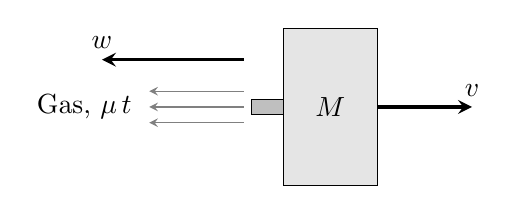
\begin{tikzpicture}[>=stealth]
 \draw[fill=gray!20] (4,0) rectangle (5.2,2);
 \node at (4.6,1) {$M$};
 \draw[fill=gray!50] (3.6,0.9) rectangle (4,1.1);
 \foreach \y in {0.8,1,1.2} \draw[->, gray] (3.5,\y) -- (2.3,\y);
 \node[anchor=east] at (2.2,1) {Gas, $\mu\,t$};
 \draw[->, very thick] (3.5,1.6) -- (1.7,1.6) node[above] {$w$};
 \draw[->, very thick] (5.2,1) -- (6.4,1) node[above] {$v$};
\end{tikzpicture}
\end{center}

Mit dem Massenstrom $\mu = \qGaO$ stösst die Pistole in der Zeit $t = \tAsO$ die Gasmasse
\begin{align}
 \Delta m &= \mGaF = \qGa\cdot\tAs = \mGa
\end{align}
aus. Astronaut und Gas waren anfänglich in Ruhe, der Gesamtimpuls bleibt null:
\begin{align}
 0 &= \left(M-\mu\,t\right)v - \mu\,t\,w
\end{align}
Damit ist
\begin{align}
 v &= \vAsF \\
   &= \frac{\mGa\cdot\wGa}{\mAs-\mGa} \\
   &= \vAs \approx \result{\vAsP{0}{2}}
\end{align}
Da der Astronaut sehr langsam bleibt, spielt es keine Rolle, dass $w$ eigentlich relativ zur Pistole gemessen wird; auch $M-\mu\,t \approx M$ würde dasselbe gerundete Resultat geben.
